\documentclass[journal]{IEEEtran}
\usepackage[a5paper, margin=10mm, onecolumn]{geometry}
\usepackage{amsmath,amssymb,amsfonts,amsthm}
\usepackage{gvv-book}
\usepackage{gvv}
\usepackage{hyperref}

\begin{document}

\title{4.7.43}
\author{Puni Aditya - EE25BTECH11046}
\maketitle

\textbf{Question:}

Show that the points $\brak{\hat{i}-\hat{j}+3\hat{k}}$ and $3\brak{\hat{i}+\hat{j}+\hat{k}}$ are equidistant from the plane $\vec{r}\cdot\brak{5\hat{i}+2\hat{j}-7\hat{k}} + 9 = 0$ and lie on opposite sides of it.

\textbf{Solution:}

Let the given points be $\vec{P_1} = \myvec{1 \\ -1 \\ 3}$ and $\vec{P_2} = \myvec{3 \\ 3 \\ 3}$.
The equation of the given plane is
\begin{align}
    \myvec{5 & 2 & -7}\vec{x} + 9 = 0
\end{align}
This can be written in the standard form $\vec{n}^\top\vec{x} = k$. Here, $\vec{n} = \myvec{5 \\ 2 \\ -7}$ and $k = -9$.
\begin{align}
    \myvec{5 & 2 & -7}\vec{x} = -9 \label{eq:plane_eqn}
\end{align}

The reflection of point $\vec{Q}$ with respect to the plane $\vec{n}^\top\vec{x}=k$ is given by
\begin{align}
    \vec{R} = \vec{Q} - \frac{2\brak{\vec{n}^\top\vec{Q}-k}}{\norm{\vec{n}}^2}\vec{n}
\end{align}

Let the reflection of point $\vec{P_1}$ with respect to the plane be $\vec{Q}$.
\begin{align}
    \vec{Q} &= \vec{P_1} - \frac{2\brak{\vec{n}^\top\vec{P_1}-k}}{\norm{\vec{n}}^2}\vec{n} \\
    &= \myvec{1 \\ -1 \\ 3} - \frac{2\brak{\myvec{5 & 2 & -7}\myvec{1 \\ -1 \\ 3} - \brak{-9}}}{5^2 + 2^2 + \brak{-7}^2}\myvec{5 \\ 2 \\ -7} \\
    &= \myvec{1 \\ -1 \\ 3} - \frac{-18}{78}\myvec{5 \\ 2 \\ -7} \\
    &= \myvec{1 \\ -1 \\ 3} + \frac{3}{13}\myvec{5 \\ 2 \\ -7} \\
    &= \myvec{\frac{28}{13} \\ -\frac{7}{13} \\ \frac{18}{13}}
\end{align}

Let a plane parallel to given plane pass through $\vec{P_1}$. Let this be $\vec{n}^\top\vec{x}=c$
\begin{align}
    \vec{n}^\top\vec{Q} &= c \\
    \myvec{5 & 2 & -7}\myvec{\frac{28}{13} \\ -\frac{7}{13} \\ \frac{18}{13}} &= c \\
    c &= \frac{140}{13}-\frac{14}{13}-\frac{126}{13} \\
    c &= 0
\end{align}

\begin{align}
    \vec{n}^\top\vec{P_2} &= \myvec{5 & 2 & -7}\myvec{3 \\ 3 \\ 3} \\
    &= 15+6-21 \\
    &= 0 = c
\end{align}

$\because \vec{P_2}\text{ lies in the plane }\vec{n}^\top\vec{x}=c$, the point $\vec{P_2}$ and $\vec{P_1}$ are equidistant from the plane $\vec{n}^\top\vec{x} = k$ and lie on the opposite sides of the plane.

\begin{figure}[h!]
    \centering
    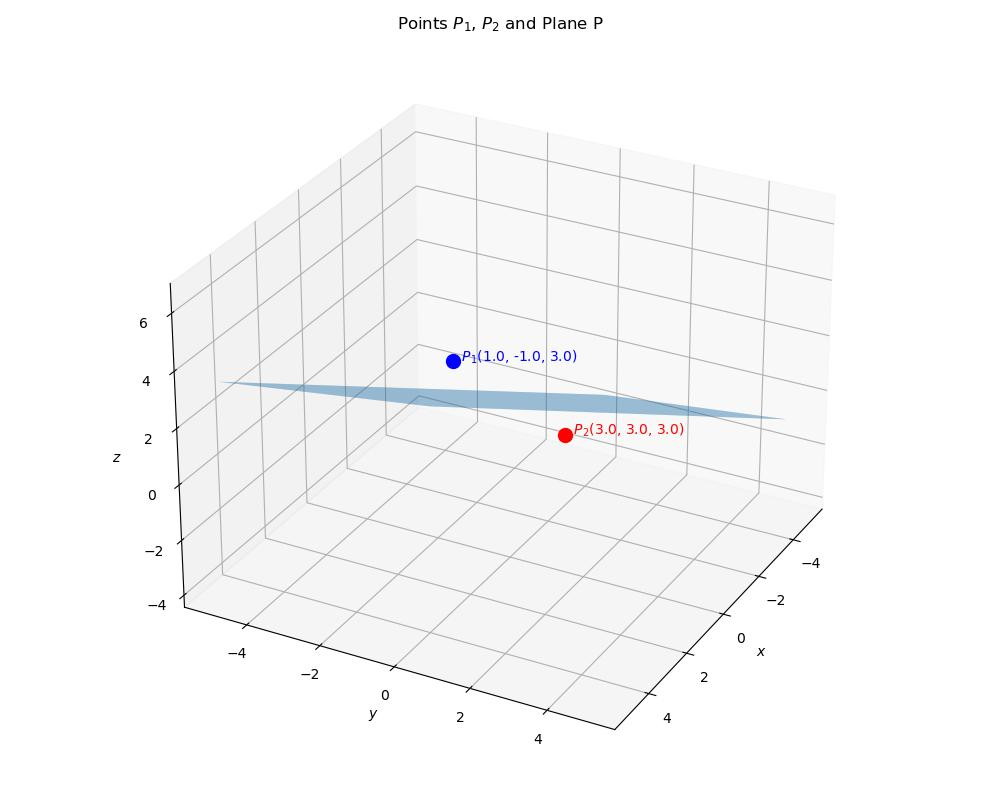
\includegraphics[width=0.75\columnwidth]{figs/plot_c.jpg}
    \caption*{Plot}
    \label{fig:fig}
\end{figure}

\end{document}
